\documentclass[aspectratio=169]{beamer}
\usepackage[utf8]{inputenc}

% design
\usetheme{CambridgeUS}
\usecolortheme{beaver}
\setbeamertemplate{itemize items}[square]
\usenavigationsymbolstemplate{\beamertemplatenavigationsymbolsempty}
\definecolor{darkred}{rgb}{0.8,0,0}
\setbeamertemplate{enumerate item}{\color{darkred}\insertenumlabel.}
\setbeamertemplate{itemize item}{\color{darkred}$\blacktriangleright$}
\setlength{\tabcolsep}{12pt}
\setbeamercolor{block title}{fg=darkred}

% bibliography
%\usepackage[backend=biber, style=authortitle]{biblatex}
\usepackage{natbib}
\usepackage{har2nat}
\bibliographystyle{unsrt}
%\addbibresource{../../smc.bib}
\usepackage{bibentry}
\nobibliography*

% tikz
\usepackage{tikz}
\usetikzlibrary{positioning}

% maths
\usepackage{amsmath}
\usepackage{amssymb}
\usepackage{amsfonts}
\usepackage{amsthm}
\theoremstyle{definition}
\newtheorem{defn}{Definition}

% useful math symbols
\newcommand{\PR}{\mathbb{P}}
\newcommand{\E}{\mathbb{E}}
\newcommand{\V}{\operatorname{Var}}
\newcommand{\eqdist}{\overset{d}{=}}
\newcommand{\I}[1]{\mathbb{I}\{#1\}}
\newcommand{\Ntoinfty}{\overset{N\to\infty}{\longrightarrow}}
\newcommand{\limNtoinfty}{\underset{N\to\infty}{\lim}}
\newcommand\indep{\protect\mathpalette{\protect\independenT}{\perp}}
\def\independenT#1#2{\mathrel{\rlap{$#1#2$}\mkern2mu{#1#2}}}

% distributions
\newcommand{\N}{\mathcal{N}}
\newcommand{\Cat}{\operatorname{Categorical}}
\newcommand{\Unif}{\operatorname{Uniform}}
\newcommand{\Mn}{\operatorname{Multinomial}}
\newcommand{\Bin}{\operatorname{Binomial}}

% project-specific commands
\newcommand{\F}{\mathcal{F}_{t-1}}
\newcommand{\vt}[2][t]{\nu_{#1}^{(#2)}}
%\newcommand{\vt}[1]{v_{#1}}
\newcommand{\wt}[2][t]{w_{#1}^{(#2)}}
%\newcommand{\wt}[1]{w_{#1}}
%\newcommand{\wbar}[2][t]{\bar{w}_{#1}^{(#2)}}
%\newcommand{\vttilde}[2][t]{\tilde{v}_{#1}^{(#2)}}
\newcommand{\Et}{\mathbb{E}_{t}}

\title[Genealogies of SMC Algorithms]{Asymptotic genealogies of sequential Monte Carlo algorithms}
\author[Suzie Brown]{\textbf{Suzie Brown} \\ University of Warwick \\ with Paul Jenkins, Adam Johansen \& Jere Koskela}
\date{18 November 2020} 

\begin{document}
\begin{frame}
\maketitle
\end{frame}

\begin{frame}{Outline}
\begin{enumerate}
\item Sequential Monte Carlo
\item Resampling and degeneracy
\item SMC genealogies
\item Examples
\end{enumerate}
\end{frame}


\begin{frame}{Sequential Monte Carlo}
Iterate these steps:
\begin{enumerate}
\item \textbf{Mutate} particles via Markov transition density $q_t$
\item \textbf{Weight} particles by potential function $g_t$
\item \textbf{Resample} particles in proportion to their weights
\end{enumerate}
\end{frame}


\begin{frame}{Resampling}
\begin{columns}
\begin{column}{0.45\textwidth}
\onslide<1->
Stochastically map continuous weights $(\wt{1}, \dots, \wt{N})$ to discrete offspring counts $(\vt{1},\dots, \vt{N})$\\[10pt]
\onslide<2->
Properties:
\begin{itemize}
\item Number of particles constant $\sum_{i=1}^N \vt{i} =N$
\item Equal weights after resampling $w_{t+}^{(i)} = 1/N$
\item Unbiased\\ $\E[\vt{i} | \wt{i}] = N\wt{i}$
\end{itemize}

\end{column}
\begin{column}{0.45\textwidth}
\centering
\onslide<1->
\includegraphics[width=\textwidth]{resample1.pdf} \\
\includegraphics[width=\textwidth]{resample2.pdf}
\end{column}
\end{columns}
\end{frame}


\begin{frame}{Resampling induces a genealogy}
\centering
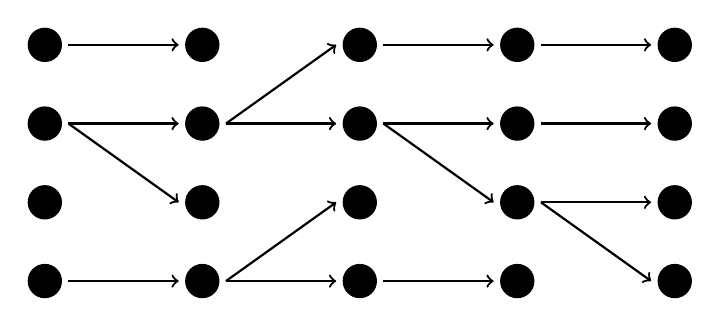
\begin{tikzpicture}
\filldraw (0,0) circle (6pt);
\filldraw (0,-1) circle (6pt);
\filldraw (0,-2) circle (6pt);
\filldraw (0,-3) circle (6pt);

\draw[->, thick] (0.3,0)--(1.7,0);
\draw[->, thick] (0.3,-1)--(1.7,-1);
\draw[->, thick] (0.3,-3)--(1.7,-3);
\draw[->, thick] (0.3,-1)--(1.7,-2);

\filldraw (2,0) circle (6pt);
\filldraw (2,-1) circle (6pt);
\filldraw (2,-2) circle (6pt);
\filldraw (2,-3) circle (6pt);

\pause

\filldraw (4,0) circle (6pt);
\filldraw (4,-1) circle (6pt);
\filldraw (4,-2) circle (6pt);
\filldraw (4,-3) circle (6pt);

\filldraw (6,0) circle (6pt);
\filldraw (6,-1) circle (6pt);
\filldraw (6,-2) circle (6pt);
\filldraw (6,-3) circle (6pt);

\filldraw (8,0) circle (6pt);
\filldraw (8,-1) circle (6pt);
\filldraw (8,-2) circle (6pt);
\filldraw (8,-3) circle (6pt);

\draw[->, thick] (2.3,-1)--(3.7,0);
\draw[->, thick] (2.3,-1)--(3.7,-1);
\draw[->, thick] (2.3,-3)--(3.7,-2);
\draw[->, thick] (2.3,-3)--(3.7,-3);

\draw[->, thick] (4.3,0)--(5.7,0);
\draw[->, thick] (4.3,-1)--(5.7,-1);
\draw[->, thick] (4.3,-1)--(5.7,-2);
\draw[->, thick] (4.3,-3)--(5.7,-3);

\draw[->, thick] (6.3,0)--(7.7,0);
\draw[->, thick] (6.3,-1)--(7.7,-1);
\draw[->, thick] (6.3,-2)--(7.7,-2);
\draw[->, thick] (6.3,-2)--(7.7,-3);
\end{tikzpicture}
\end{frame}


\begin{frame}{Resampling induces a genealogy}
\centering
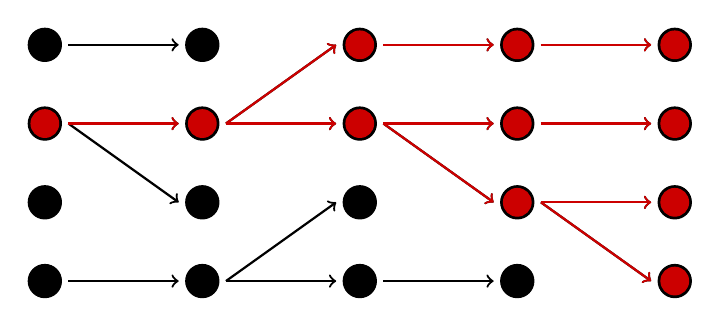
\begin{tikzpicture}
\filldraw (0,0) circle (6pt);
\filldraw (0,-1) circle (6pt);
\filldraw (0,-2) circle (6pt);
\filldraw (0,-3) circle (6pt);

\draw[->, thick] (0.3,0)--(1.7,0);
\draw[->, thick] (0.3,-1)--(1.7,-1);
\draw[->, thick] (0.3,-3)--(1.7,-3);
\draw[->, thick] (0.3,-1)--(1.7,-2);

\filldraw (2,0) circle (6pt);
\filldraw (2,-1) circle (6pt);
\filldraw (2,-2) circle (6pt);
\filldraw (2,-3) circle (6pt);

\filldraw (4,0) circle (6pt);
\filldraw (4,-1) circle (6pt);
\filldraw (4,-2) circle (6pt);
\filldraw (4,-3) circle (6pt);

\filldraw (6,0) circle (6pt);
\filldraw (6,-1) circle (6pt);
\filldraw (6,-2) circle (6pt);
\filldraw (6,-3) circle (6pt);

\filldraw (8,0) circle (6pt);
\filldraw (8,-1) circle (6pt);
\filldraw (8,-2) circle (6pt);
\filldraw (8,-3) circle (6pt);

\draw[->, thick] (2.3,-1)--(3.7,0);
\draw[->, thick] (2.3,-1)--(3.7,-1);
\draw[->, thick] (2.3,-3)--(3.7,-2);
\draw[->, thick] (2.3,-3)--(3.7,-3);

\draw[->, thick] (4.3,0)--(5.7,0);
\draw[->, thick] (4.3,-1)--(5.7,-1);
\draw[->, thick] (4.3,-1)--(5.7,-2);
\draw[->, thick] (4.3,-3)--(5.7,-3);

\draw[->, thick] (6.3,0)--(7.7,0);
\draw[->, thick] (6.3,-1)--(7.7,-1);
\draw[->, thick] (6.3,-2)--(7.7,-2);
\draw[->, thick] (6.3,-2)--(7.7,-3);

% highlight first lineage
\filldraw[darkred] (8,0) circle (5pt);
\pause
\filldraw[darkred] (6,0) circle (5pt);
\filldraw[darkred] (4,0) circle (5pt);
\filldraw[darkred] (2,-1) circle (5pt);
\filldraw[darkred] (0,-1) circle (5pt);

\draw[->, thick, darkred] (0.3,-1)--(1.7,-1);
\draw[->, thick, darkred] (2.3,-1)--(3.7,0);
\draw[->, thick, darkred] (4.3,0)--(5.7,0);
\draw[->, thick, darkred] (6.3,0)--(7.7,0);

\pause
% highlight other lineages
\filldraw[darkred] (4,-1) circle (5pt);
\filldraw[darkred] (6,-1) circle (5pt);
\filldraw[darkred] (8,-1) circle (5pt);
\filldraw[darkred] (6,-2) circle (5pt);
\filldraw[darkred] (8,-2) circle (5pt);
\filldraw[darkred] (8,-3) circle (5pt);

\draw[->, thick, darkred] (2.3,-1)--(3.7,-1);
\draw[->, thick, darkred] (4.3,-1)--(5.7,-1);
\draw[->, thick, darkred] (4.3,-1)--(5.7,-2);
\draw[->, thick, darkred] (6.3,-1)--(7.7,-1);
\draw[->, thick, darkred] (6.3,-2)--(7.7,-2);
\draw[->, thick, darkred] (6.3,-2)--(7.7,-3);
\end{tikzpicture}
\end{frame}


\begin{frame}{Resampling induces a genealogy}
\vspace{1cm}

\centering
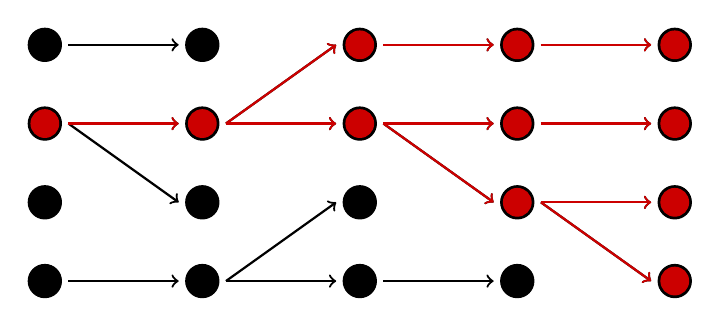
\begin{tikzpicture}
\filldraw (0,0) circle (6pt);
\filldraw (0,-1) circle (6pt);
\filldraw (0,-2) circle (6pt);
\filldraw (0,-3) circle (6pt);

\draw[->, thick] (0.3,0)--(1.7,0);
\draw[->, thick] (0.3,-1)--(1.7,-1);
\draw[->, thick] (0.3,-3)--(1.7,-3);
\draw[->, thick] (0.3,-1)--(1.7,-2);

\filldraw (2,0) circle (6pt);
\filldraw (2,-1) circle (6pt);
\filldraw (2,-2) circle (6pt);
\filldraw (2,-3) circle (6pt);

\filldraw (4,0) circle (6pt);
\filldraw (4,-1) circle (6pt);
\filldraw (4,-2) circle (6pt);
\filldraw (4,-3) circle (6pt);

\filldraw (6,0) circle (6pt);
\filldraw (6,-1) circle (6pt);
\filldraw (6,-2) circle (6pt);
\filldraw (6,-3) circle (6pt);

\filldraw (8,0) circle (6pt);
\filldraw (8,-1) circle (6pt);
\filldraw (8,-2) circle (6pt);
\filldraw (8,-3) circle (6pt);

\draw[->, thick] (2.3,-1)--(3.7,0);
\draw[->, thick] (2.3,-1)--(3.7,-1);
\draw[->, thick] (2.3,-3)--(3.7,-2);
\draw[->, thick] (2.3,-3)--(3.7,-3);

\draw[->, thick] (4.3,0)--(5.7,0);
\draw[->, thick] (4.3,-1)--(5.7,-1);
\draw[->, thick] (4.3,-1)--(5.7,-2);
\draw[->, thick] (4.3,-3)--(5.7,-3);

\draw[->, thick] (6.3,0)--(7.7,0);
\draw[->, thick] (6.3,-1)--(7.7,-1);
\draw[->, thick] (6.3,-2)--(7.7,-2);
\draw[->, thick] (6.3,-2)--(7.7,-3);

% highlight first lineage
\filldraw[darkred] (8,0) circle (5pt);
\filldraw[darkred] (6,0) circle (5pt);
\filldraw[darkred] (4,0) circle (5pt);
\filldraw[darkred] (2,-1) circle (5pt);
\filldraw[darkred] (0,-1) circle (5pt);

\draw[->, thick, darkred] (0.3,-1)--(1.7,-1);
\draw[->, thick, darkred] (2.3,-1)--(3.7,0);
\draw[->, thick, darkred] (4.3,0)--(5.7,0);
\draw[->, thick, darkred] (6.3,0)--(7.7,0);

% highlight other lineages
\filldraw[darkred] (4,-1) circle (5pt);
\filldraw[darkred] (6,-1) circle (5pt);
\filldraw[darkred] (8,-1) circle (5pt);
\filldraw[darkred] (6,-2) circle (5pt);
\filldraw[darkred] (8,-2) circle (5pt);
\filldraw[darkred] (8,-3) circle (5pt);

\draw[->, thick, darkred] (2.3,-1)--(3.7,-1);
\draw[->, thick, darkred] (4.3,-1)--(5.7,-1);
\draw[->, thick, darkred] (4.3,-1)--(5.7,-2);
\draw[->, thick, darkred] (6.3,-1)--(7.7,-1);
\draw[->, thick, darkred] (6.3,-2)--(7.7,-2);
\draw[->, thick, darkred] (6.3,-2)--(7.7,-3);
\end{tikzpicture}

\vspace{1cm}
\textbf{Ancestral degeneracy:} for $t<<T$, few distinct samples are available
\end{frame}


\begin{frame}{Encoding genealogies}
\begin{itemize}
\item Label time in reverse
\item Population of $N$ particles
\item Sample $n\leq N$ terminal particles
\item Describe genealogy by stochastic process $(G_t^{(n,N)})_{t\in\mathbb{N}_0}$ on space of partitions of $\{1,\dots,n\}$
\item Elements $i, j$ are in the same block of the partition $G_t^{(n,N)}$ iff particles $i$ and $j$ share a common ancestor at time $t$
\item Initially $G_0^{(n,N)} = \{ \{1\}, \dots, \{n\} \}$
\item The only possible non-identity transitions are those that merge blocks
\item The trivial partition $\{ \{ 1,\dots, n \} \}$ is an absorbing state
\end{itemize}
\end{frame}


\begin{frame}{Encoding genealogies} %%% add some pauses in here
\centering
\begin{tikzpicture}
\draw[dotted] (0,-4.5)--(0,0.5);
\draw[dotted] (2,-4.5)--(2,0.5);
\draw[dotted] (4,-4.5)--(4,0.5);
\draw[dotted] (6,-4.5)--(6,0.5);
\draw[dotted] (8,-4.5)--(8,0.5);

\draw[thick, darkred] (0,-1)--(2,-1);
\draw[thick, darkred] (2,0)--(2,-2);
\draw[thick, darkred] (2,0)--(8,0);
\draw[thick, darkred] (2,-2)--(4,-2);
\draw[thick, darkred] (4,-3)--(4,-1);
\draw[thick, darkred] (4,-1)--(8,-1);
\draw[thick, darkred] (4,-3)--(6,-3);
\draw[thick, darkred] (6,-2)--(6,-4);
\draw[thick, darkred] (6,-2)--(8,-2);
\draw[thick, darkred] (6,-4)--(8,-4);

\pause

\node at (8.3,0) {1};
\node at (8.3,-1) {2};
\node at (8.3,-2) {3};
\node at (8.3,-4) {4};

\node at (8,-4.8) {$t=0$};
\node at (8,-5.5) {$\{1\}, \{2\},\{3\}, \{4\}$};
\end{tikzpicture}
\end{frame}

\begin{frame}{Encoding genealogies}
\centering
\begin{tikzpicture}
\draw[dotted] (0,-4.5)--(0,0.5);
\draw[dotted] (2,-4.5)--(2,0.5);
\draw[dotted] (4,-4.5)--(4,0.5);
\draw[dotted] (6,-4.5)--(6,0.5);
\draw[dotted] (8,-4.5)--(8,0.5);

\draw[thick, darkred] (0,-1)--(2,-1);
\draw[thick, darkred] (2,0)--(2,-2);
\draw[thick, darkred] (2,0)--(8,0);
\draw[thick, darkred] (2,-2)--(4,-2);
\draw[thick, darkred] (4,-3)--(4,-1);
\draw[thick, darkred] (4,-1)--(8,-1);
\draw[thick, darkred] (4,-3)--(6,-3);
\draw[thick, darkred] (6,-2)--(6,-4);
\draw[thick, darkred] (6,-2)--(8,-2);
\draw[thick, darkred] (6,-4)--(8,-4);

\node at (8.3,0) {1};
\node at (8.3,-1) {2};
\node at (8.3,-2) {3};
\node at (8.3,-4) {4};

\node at (6,-4.8) {$t=1$};
\node at (6,-5.5) {$\{1\}, \{2\},\{3,4\}$};
\end{tikzpicture}
\end{frame}

\begin{frame}{Encoding genealogies}
\centering
\begin{tikzpicture}
\draw[dotted] (0,-4.5)--(0,0.5);
\draw[dotted] (2,-4.5)--(2,0.5);
\draw[dotted] (4,-4.5)--(4,0.5);
\draw[dotted] (6,-4.5)--(6,0.5);
\draw[dotted] (8,-4.5)--(8,0.5);

\draw[thick, darkred] (0,-1)--(2,-1);
\draw[thick, darkred] (2,0)--(2,-2);
\draw[thick, darkred] (2,0)--(8,0);
\draw[thick, darkred] (2,-2)--(4,-2);
\draw[thick, darkred] (4,-3)--(4,-1);
\draw[thick, darkred] (4,-1)--(8,-1);
\draw[thick, darkred] (4,-3)--(6,-3);
\draw[thick, darkred] (6,-2)--(6,-4);
\draw[thick, darkred] (6,-2)--(8,-2);
\draw[thick, darkred] (6,-4)--(8,-4);

\node at (8.3,0) {1};
\node at (8.3,-1) {2};
\node at (8.3,-2) {3};
\node at (8.3,-4) {4};

\node at (4,-4.8) {$t=2$};
\node at (4,-5.5) {$\{1\}, \{2,3,4\}$};
\end{tikzpicture}
\end{frame}

\begin{frame}{Encoding genealogies}
\centering
\begin{tikzpicture}
\draw[dotted] (0,-4.5)--(0,0.5);
\draw[dotted] (2,-4.5)--(2,0.5);
\draw[dotted] (4,-4.5)--(4,0.5);
\draw[dotted] (6,-4.5)--(6,0.5);
\draw[dotted] (8,-4.5)--(8,0.5);

\draw[thick, darkred] (0,-1)--(2,-1);
\draw[thick, darkred] (2,0)--(2,-2);
\draw[thick, darkred] (2,0)--(8,0);
\draw[thick, darkred] (2,-2)--(4,-2);
\draw[thick, darkred] (4,-3)--(4,-1);
\draw[thick, darkred] (4,-1)--(8,-1);
\draw[thick, darkred] (4,-3)--(6,-3);
\draw[thick, darkred] (6,-2)--(6,-4);
\draw[thick, darkred] (6,-2)--(8,-2);
\draw[thick, darkred] (6,-4)--(8,-4);

\node at (8.3,0) {1};
\node at (8.3,-1) {2};
\node at (8.3,-2) {3};
\node at (8.3,-4) {4};

\node at (2,-4.8) {$t=3$};
\node at (2,-5.5) {$\{1,2,3,4\}$};
\end{tikzpicture}
\end{frame}


\begin{frame}{Kingman's $n$-coalescent}
\begin{columns}
\begin{column}{0.45\textwidth}
\begin{itemize}
\item Continuous-time Markov chain on the space of partitions of $\{1,\dots,n\}$
\item Single pair mergers only
\item Each pair merges independently at rate 1 (total merge rate $\binom{k}{2}$ while there are $k$ distinct lineages)
\end{itemize}
\end{column}
\begin{column}{0.45\textwidth}
\includegraphics[width=\textwidth]{kingman.png}
\hspace*{\fill} \tiny{image: Wikimedia commons}
\end{column}
\end{columns}
\end{frame}


\begin{frame}{Time scale}
The probability that a randomly chosen pair of particles at generation $t$ share a common ancestor at generation $(t-1)$, conditional on offspring counts, is
\begin{equation*}
c_N(t) = \frac{1}{(N)_2} \sum_{i=1}^N (\vt{i})_2
\end{equation*}
To get an $n$-coalescent, this should converge to 1 (the required pair merger rate),
so we rescale time by the inverse
\begin{equation*}
\tau_N(t) := \min\left\{ s\geq 1 : \sum_{r=1}^s c_N(r) \geq t \right\}
\end{equation*}
\end{frame}


\begin{frame}{Main theorem}
\begin{itemize}
\item Offspring counts $(\vt{1},\dots,\vt{N})$
\pause
\item Parent-offspring assignments are uniform given offspring counts
\item Time scale does not explode (i.e.\ $\PR[\tau_N(t)=\infty]=0$ for all finite $t$)
\item There exists a sequence $(b_N)$ such that $\lim_{N\to\infty} b_N = 0$ and
\begin{equation*}
\frac{1}{(N)_3} \sum_{i=1}^N \E_t [ (\vt{i})_3 ]
\leq b_N \frac{1}{(N)_2} \sum_{i=1}^N \E_t [ (\vt{i})_2 ]
\end{equation*}
\end{itemize}
\pause
Then the finite-dimensional distributions of the time-rescaled genealogies converge to Kingman's $n$-coalescent as $N\to\infty$.
\end{frame}


\begin{frame}{Corollaries}
We established the theorem in these cases:
\begin{itemize}
\item Multinomial resampling
\item Stochastic rounding 
\item Conditional SMC with multinomial resampling
\end{itemize}
\end{frame}


\begin{frame}{Multinomial resampling}
\begin{itemize}
\item Offspring counts are sampled from Multinomial distribution parametrised by weights
\item Easy to analyse, but doesn't perform well
\item (For the population geneticists): different from Wright-Fisher model because not neutral
\end{itemize}
\end{frame}

\begin{frame}{Corollary: multinomial resampling}
Consider an SMC algorithm with potential $g$ and transition density $q$, satisfying
\begin{align*}
\frac{1}{a} \leq &g_t(x, x^\prime) \leq a \\
\varepsilon h(x^\prime) \leq &q_t(x, x^\prime) \leq \frac{1}{\varepsilon} h(x^\prime) 
\end{align*}
for constants $0<\varepsilon\leq 1\leq a<\infty$, and probablity distribution $h(\cdot)$.\\[10pt]

Under multinomial resampling, the rescaled genealogies converge to Kingman's coalescent.
\end{frame}


\begin{frame}{Stochastic rounding}
$\mathbf{Y}: \mathbb{R}_+^N \to \mathbb{N}^N$ is a \emph{stochastic rounding} of $\mathbf{X}$ if for $i=1,\dots,N$
\begin{equation*}
Y_i \mid X_i =
\begin{cases}
 \lfloor X_i \rfloor & \text{with probability } 1- X_i + \lfloor X_i \rfloor \\
  \lfloor X_i \rfloor +1 & \text{with probability } X_i - \lfloor X_i \rfloor 
\end{cases}
\end{equation*}

%%% add pause
\begin{itemize}
\item We can construct low-variance resampling schemes using stochastic rounding
\item Take $X_i = N\wt{i}$ and $Y_i = \vt{i}$
\item Require further constraint $Y_1 + \cdots + Y_N = N$
\item \textbf{Examples:} systematic, residual-stratified, branching system\footnote{Crisan, Lyons. \textit{Prob Theory \& Related Fields,} 1997}, SSP resampling\footnote{Gerber, Whiteley, Chopin. \textit{Ann Stat,} 2019.}
\end{itemize}
\end{frame}


\begin{frame}{Corollary: stochastic rounding}
Consider an SMC algorithm with potential $g$ and transition density $q$, satisfying
\begin{align*}
\frac{1}{a} \leq &g_t(x, x^\prime) \leq a \\
\varepsilon h(x^\prime) \leq &q_t(x, x^\prime) \leq \frac{1}{\varepsilon} h(x^\prime) 
\end{align*}
for constants $0<\varepsilon\leq 1\leq a<\infty$, and probablity distribution $h(\cdot)$.\\[10pt]

Under stochastic rounding -based resampling, the rescaled genealogies converge to Kingman's coalescent.
\end{frame}


%%% Make illustrative diagram about CSMC
\begin{frame}{Conditional SMC}
\begin{itemize}
\item Used for SMC updates in particle MCMC\footnote{Andrieu, Doucet, Holenstein. \textit{JRSSB}, 2010.}
\item One ``immortal lineage'' is conditioned to survive all mutation and resampling steps
\item Resampling algorithm must deterministically propagate this ``immortal lineage''
\item For example: fix one offspring to immortal lineage, multinomial sampling for the remaining counts
\pause
\item Conjecture: theorem also applies to conditional SMC with stochastic rounding
\end{itemize}
\end{frame}


\begin{frame}{Corollary: conditional SMC}
Consider a conditional SMC algorithm with potential $g$ and transition density $q$, satisfying
\begin{align*}
\frac{1}{a} \leq &g_t(x, x^\prime) \leq a \\
\varepsilon h(x^\prime) \leq &q_t(x, x^\prime) \leq \frac{1}{\varepsilon} h(x^\prime) 
\end{align*}
for constants $0<\varepsilon\leq 1\leq a<\infty$, and probablity distribution $h(\cdot)$.\\[10pt]

Under multinomial resampling, the rescaled genealogies converge to Kingman's coalescent.
\end{frame}



%%% amalgamate following slides:
\begin{frame}{Summary}
\begin{itemize}
\item We consider genealogies of SMC algorithms
\item We provide simple conditions for asymptotically Kingman genealogies
\item Satisfied by stochastic rounding -based resampling
\item Satisfied by conditional SMC with multinomial resampling...
\item ... but this hides some interesting pre-limiting behaviour
\end{itemize}
\end{frame}

\begin{frame}{Open questions}
\begin{itemize}
\item Verify theorem for other important resampling schemes (stratified, residual-multinomial)
\item How to estimate the time scale $c_N$ a priori (since it depends on offspring counts)
\item Weak convergence so we can say more about convergence of expectations
\item Rates of convergence
\item Finite-$N$ behaviour
\end{itemize}
\end{frame}


\begin{frame}{In conclusion...}
\begin{itemize}
\item Genealogies can help us to analyse performance of smoothing algorithms which suffer ancestral degeneracy
\item We have simple conditions under which these genealogies converge to $n$-coalescent
\item These conditions are verified for some important classes of SMC algorithms
\end{itemize}

\pause
Open questions
\begin{itemize}
\item Verify theorem for other important resampling schemes (stratified, residual-multinomial)
\item How to estimate the time scale $c_N$ a priori (since it depends on offspring counts)
\item Weak convergence so we can say more about convergence of expectations
\item Rates of convergence
\item Finite-$N$ behaviour
\end{itemize}
\end{frame}


\end{document}